% !TeX root = document.tex
% !TeX encoding = UTF-8 Unicode

\subsection{Results}%
\label{subsec:ts-results}

\begin{slide}{Observer}
  \begin{columns}[c]
    \begin{column}{0.55\textwidth}
      \begin{align}
        A              & = \begin{bmatrix}
                             -1 & 1  & 0     & 0  & 0  \\
                             -1 & -1 & 1.495 & 0  & 0  \\
                             0  & 0  & -2    & 1  & 0  \\
                             0  & 0  & 0     & -3 & 1  \\
                             0  & 0  & 0     & 0  & -5
                           \end{bmatrix},        \\
        B              & =\begin{bmatrix}
                            0 \\ 0 \\ 0 \\ 0 \\ 16
                          \end{bmatrix},
        C = \begin{bmatrix}
              -5.517 \\ 2.759 \\ 0 \\ 0 \\ 0
            \end{bmatrix}^{\top},
        D = 0                                               \\
        \textrm{poles} & = \{-1\pm{}1\imath{}, -2, -3, -5\}
      \end{align}
    \end{column}%
    \hfill%
    \begin{column}{0.55\textwidth}
      \begin{figure}[ht!]
        \centering
        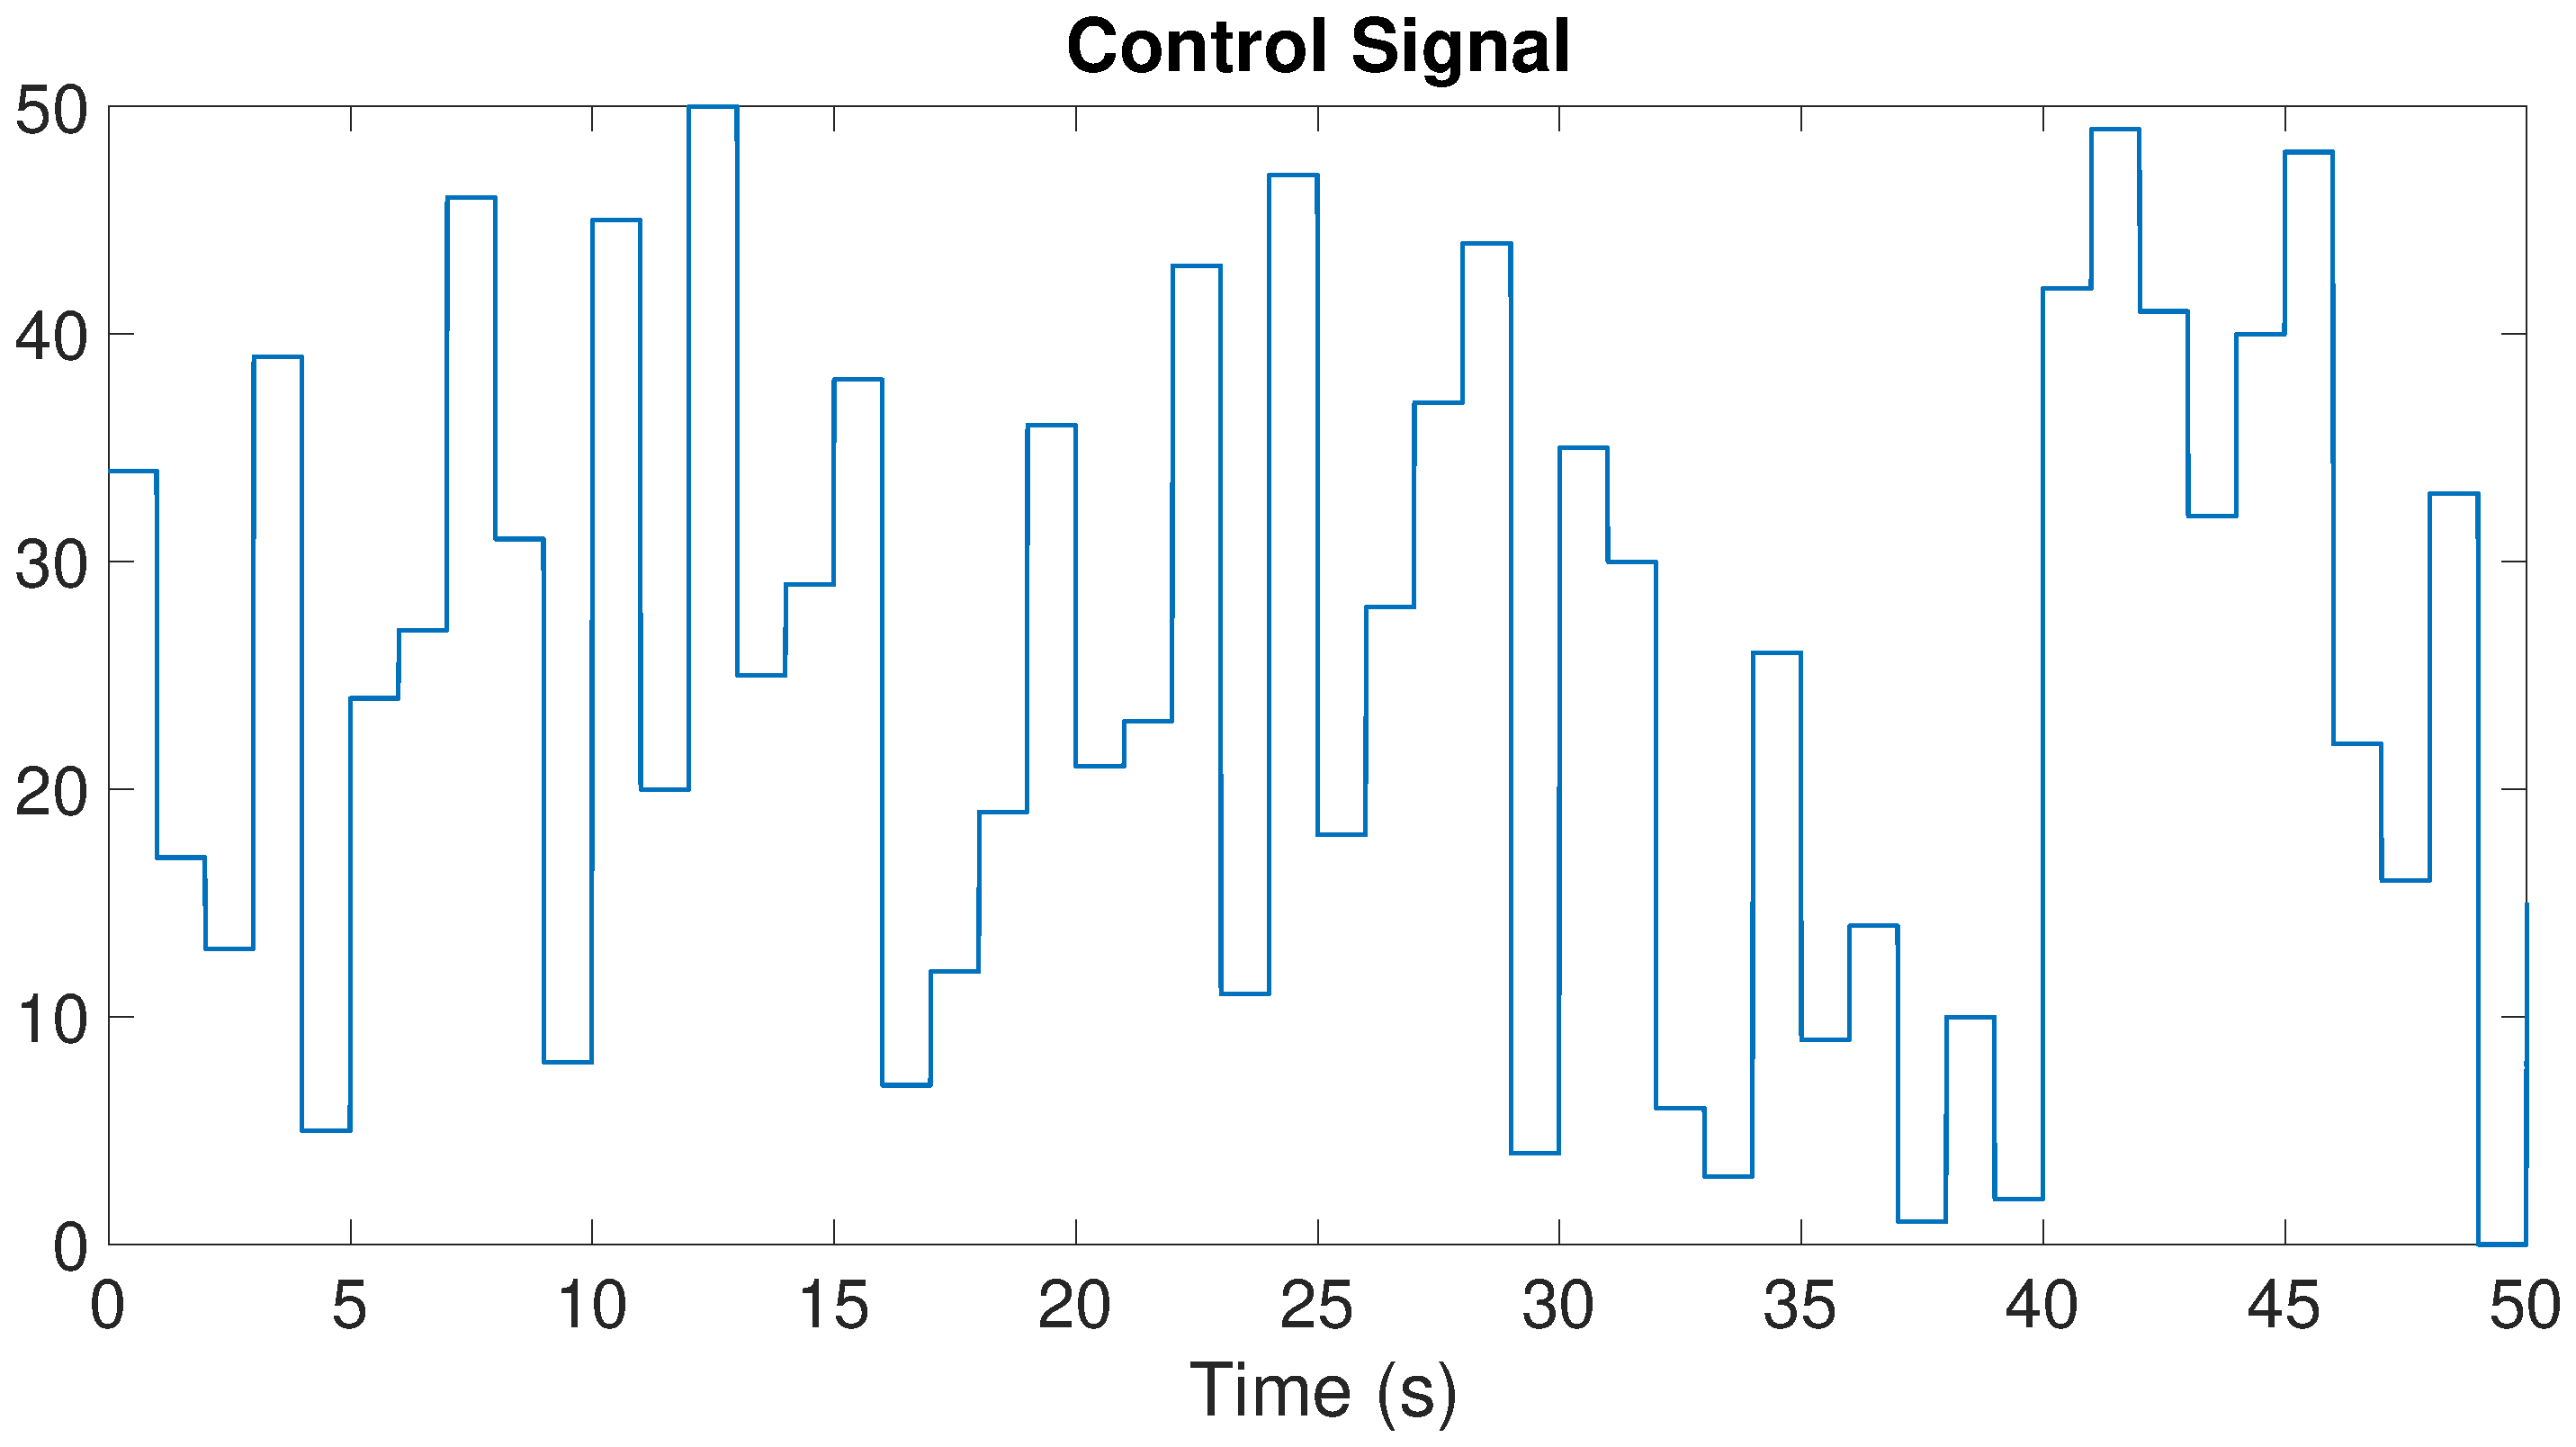
\includegraphics[width=\linewidth]{stair-input-u}
        \caption{Control Signal.}%
      \end{figure}
    \end{column}%
  \end{columns}
\end{slide}

\begin{slide}{Observer}
  \begin{columns}[c]
    \begin{column}{0.55\textwidth}
      \begin{figure}[ht!]
        \centering
        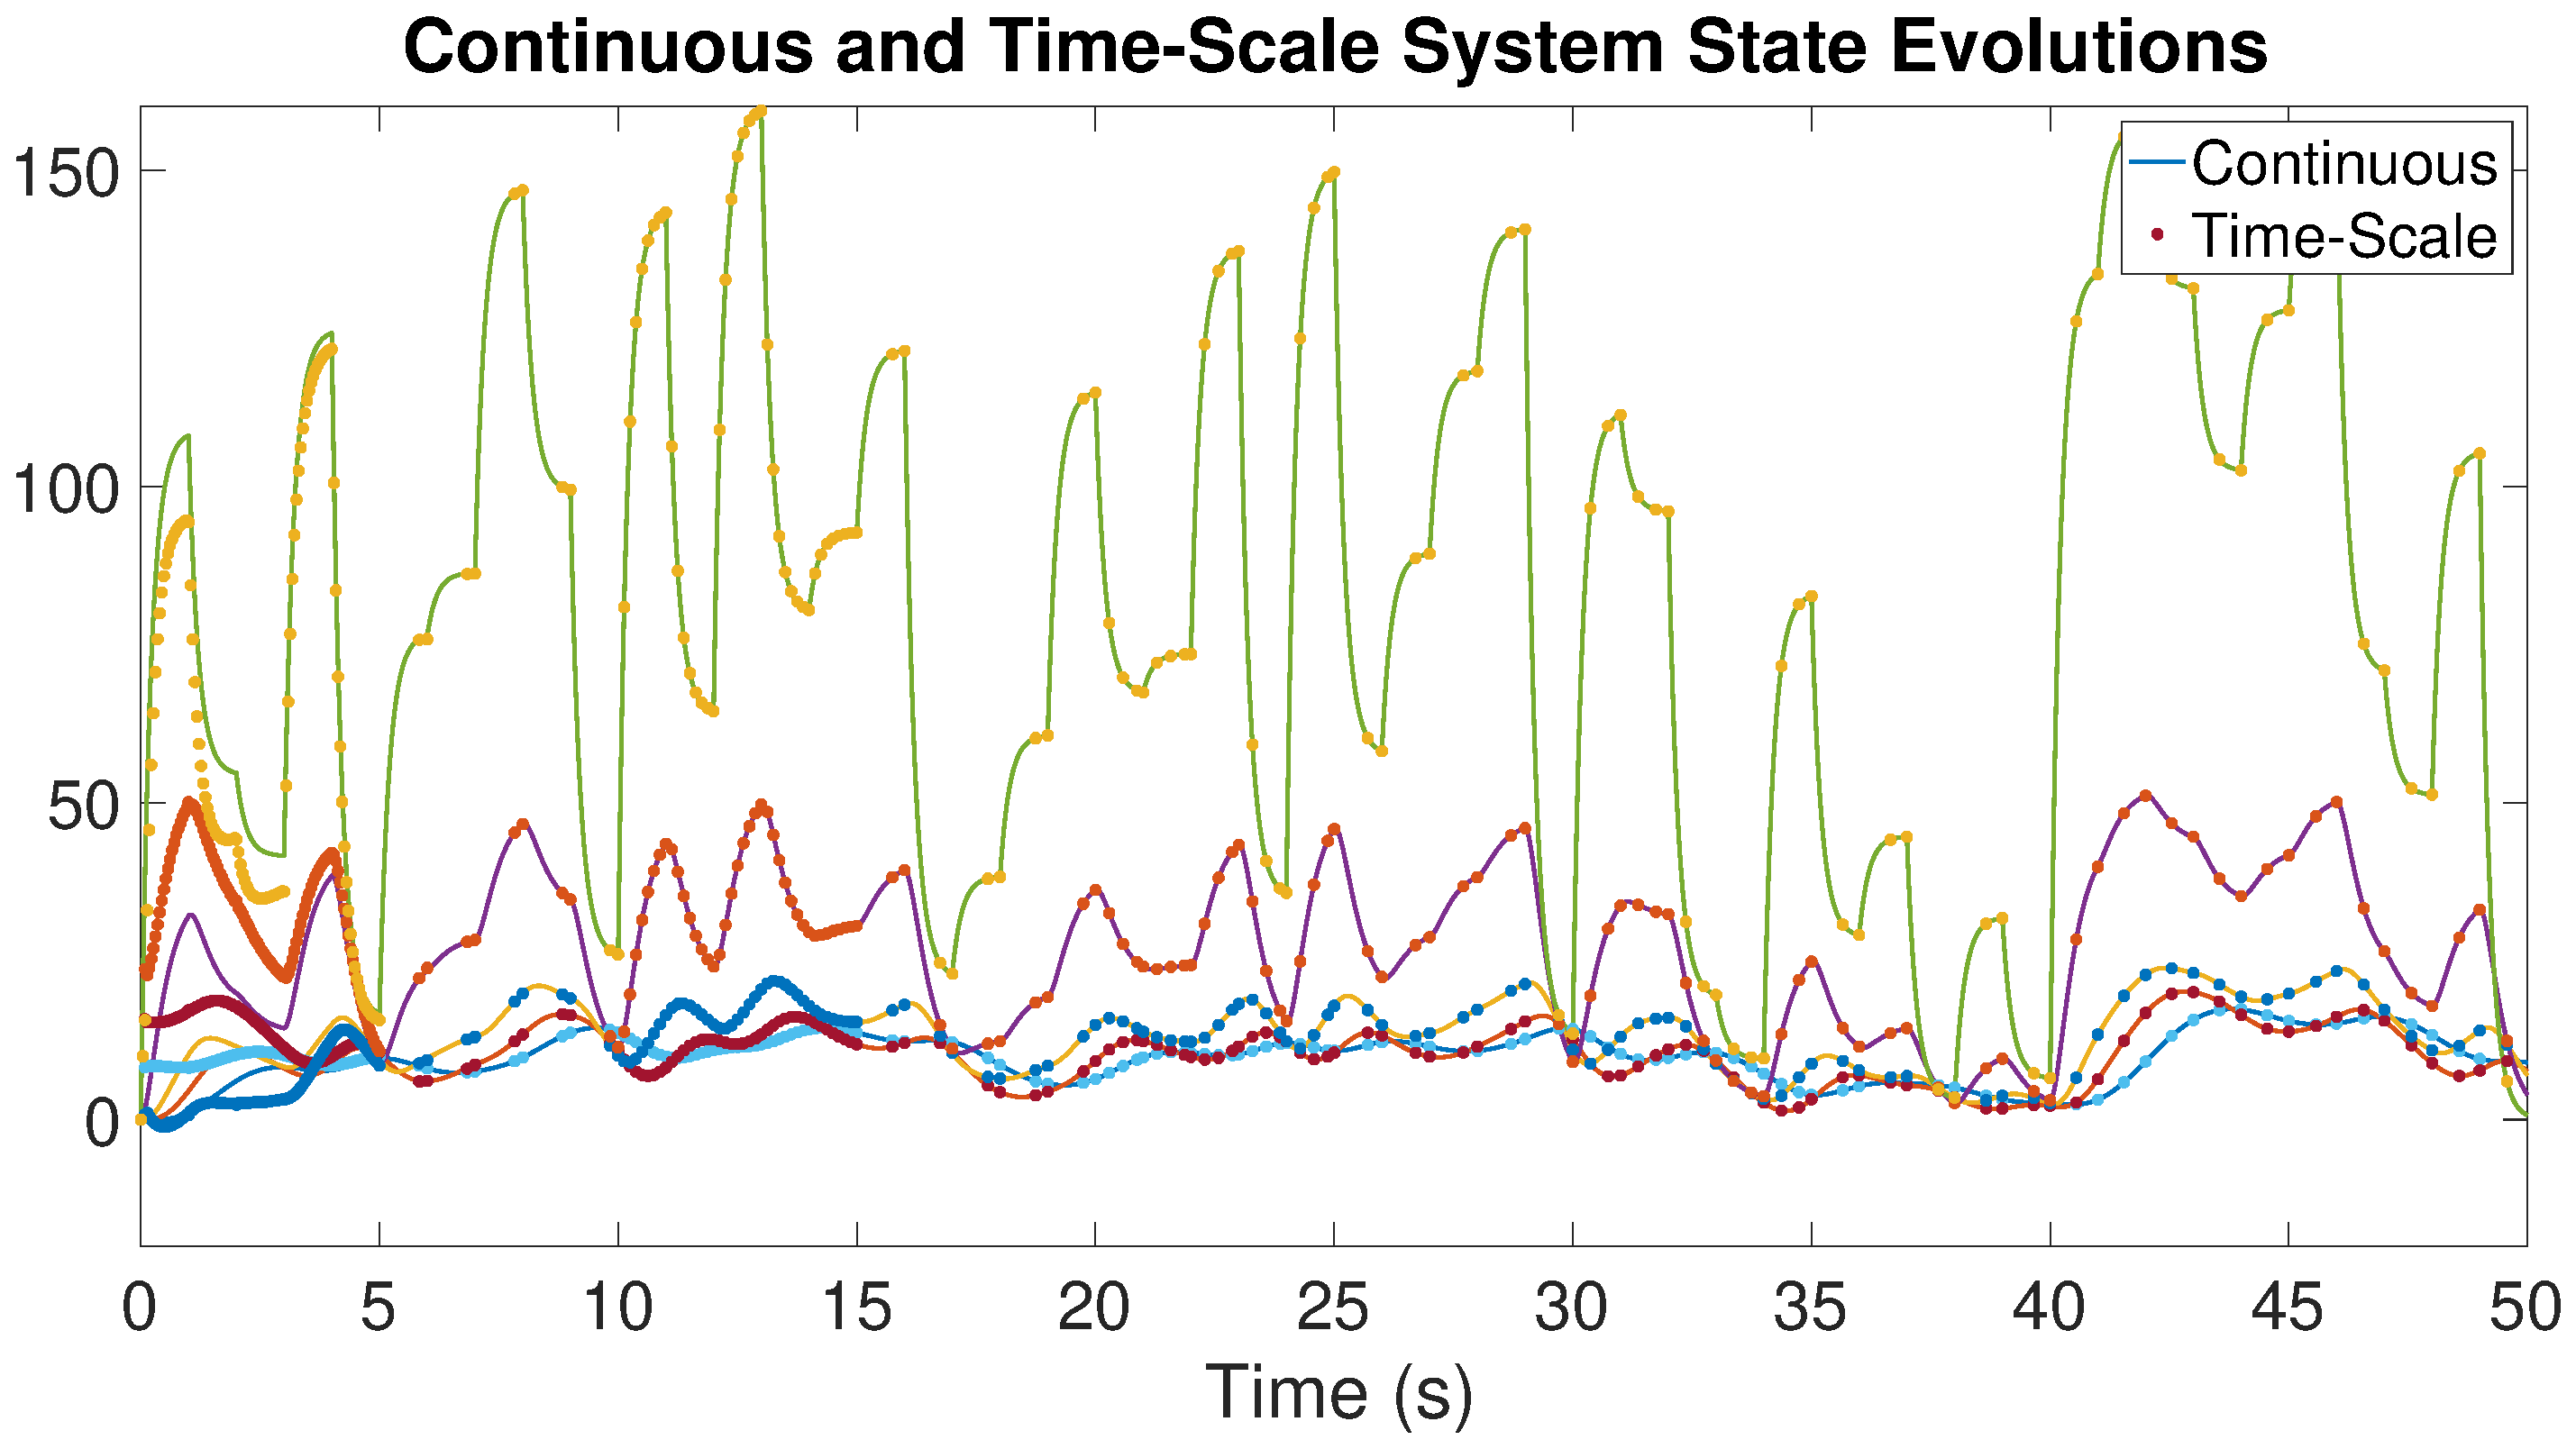
\includegraphics[width=\linewidth]{stair-input}
        \caption{Observed and system's states.}%
      \end{figure}
    \end{column}%
    \hfill%
    \begin{column}{0.55\textwidth}
      \begin{figure}[ht!]
        \centering
        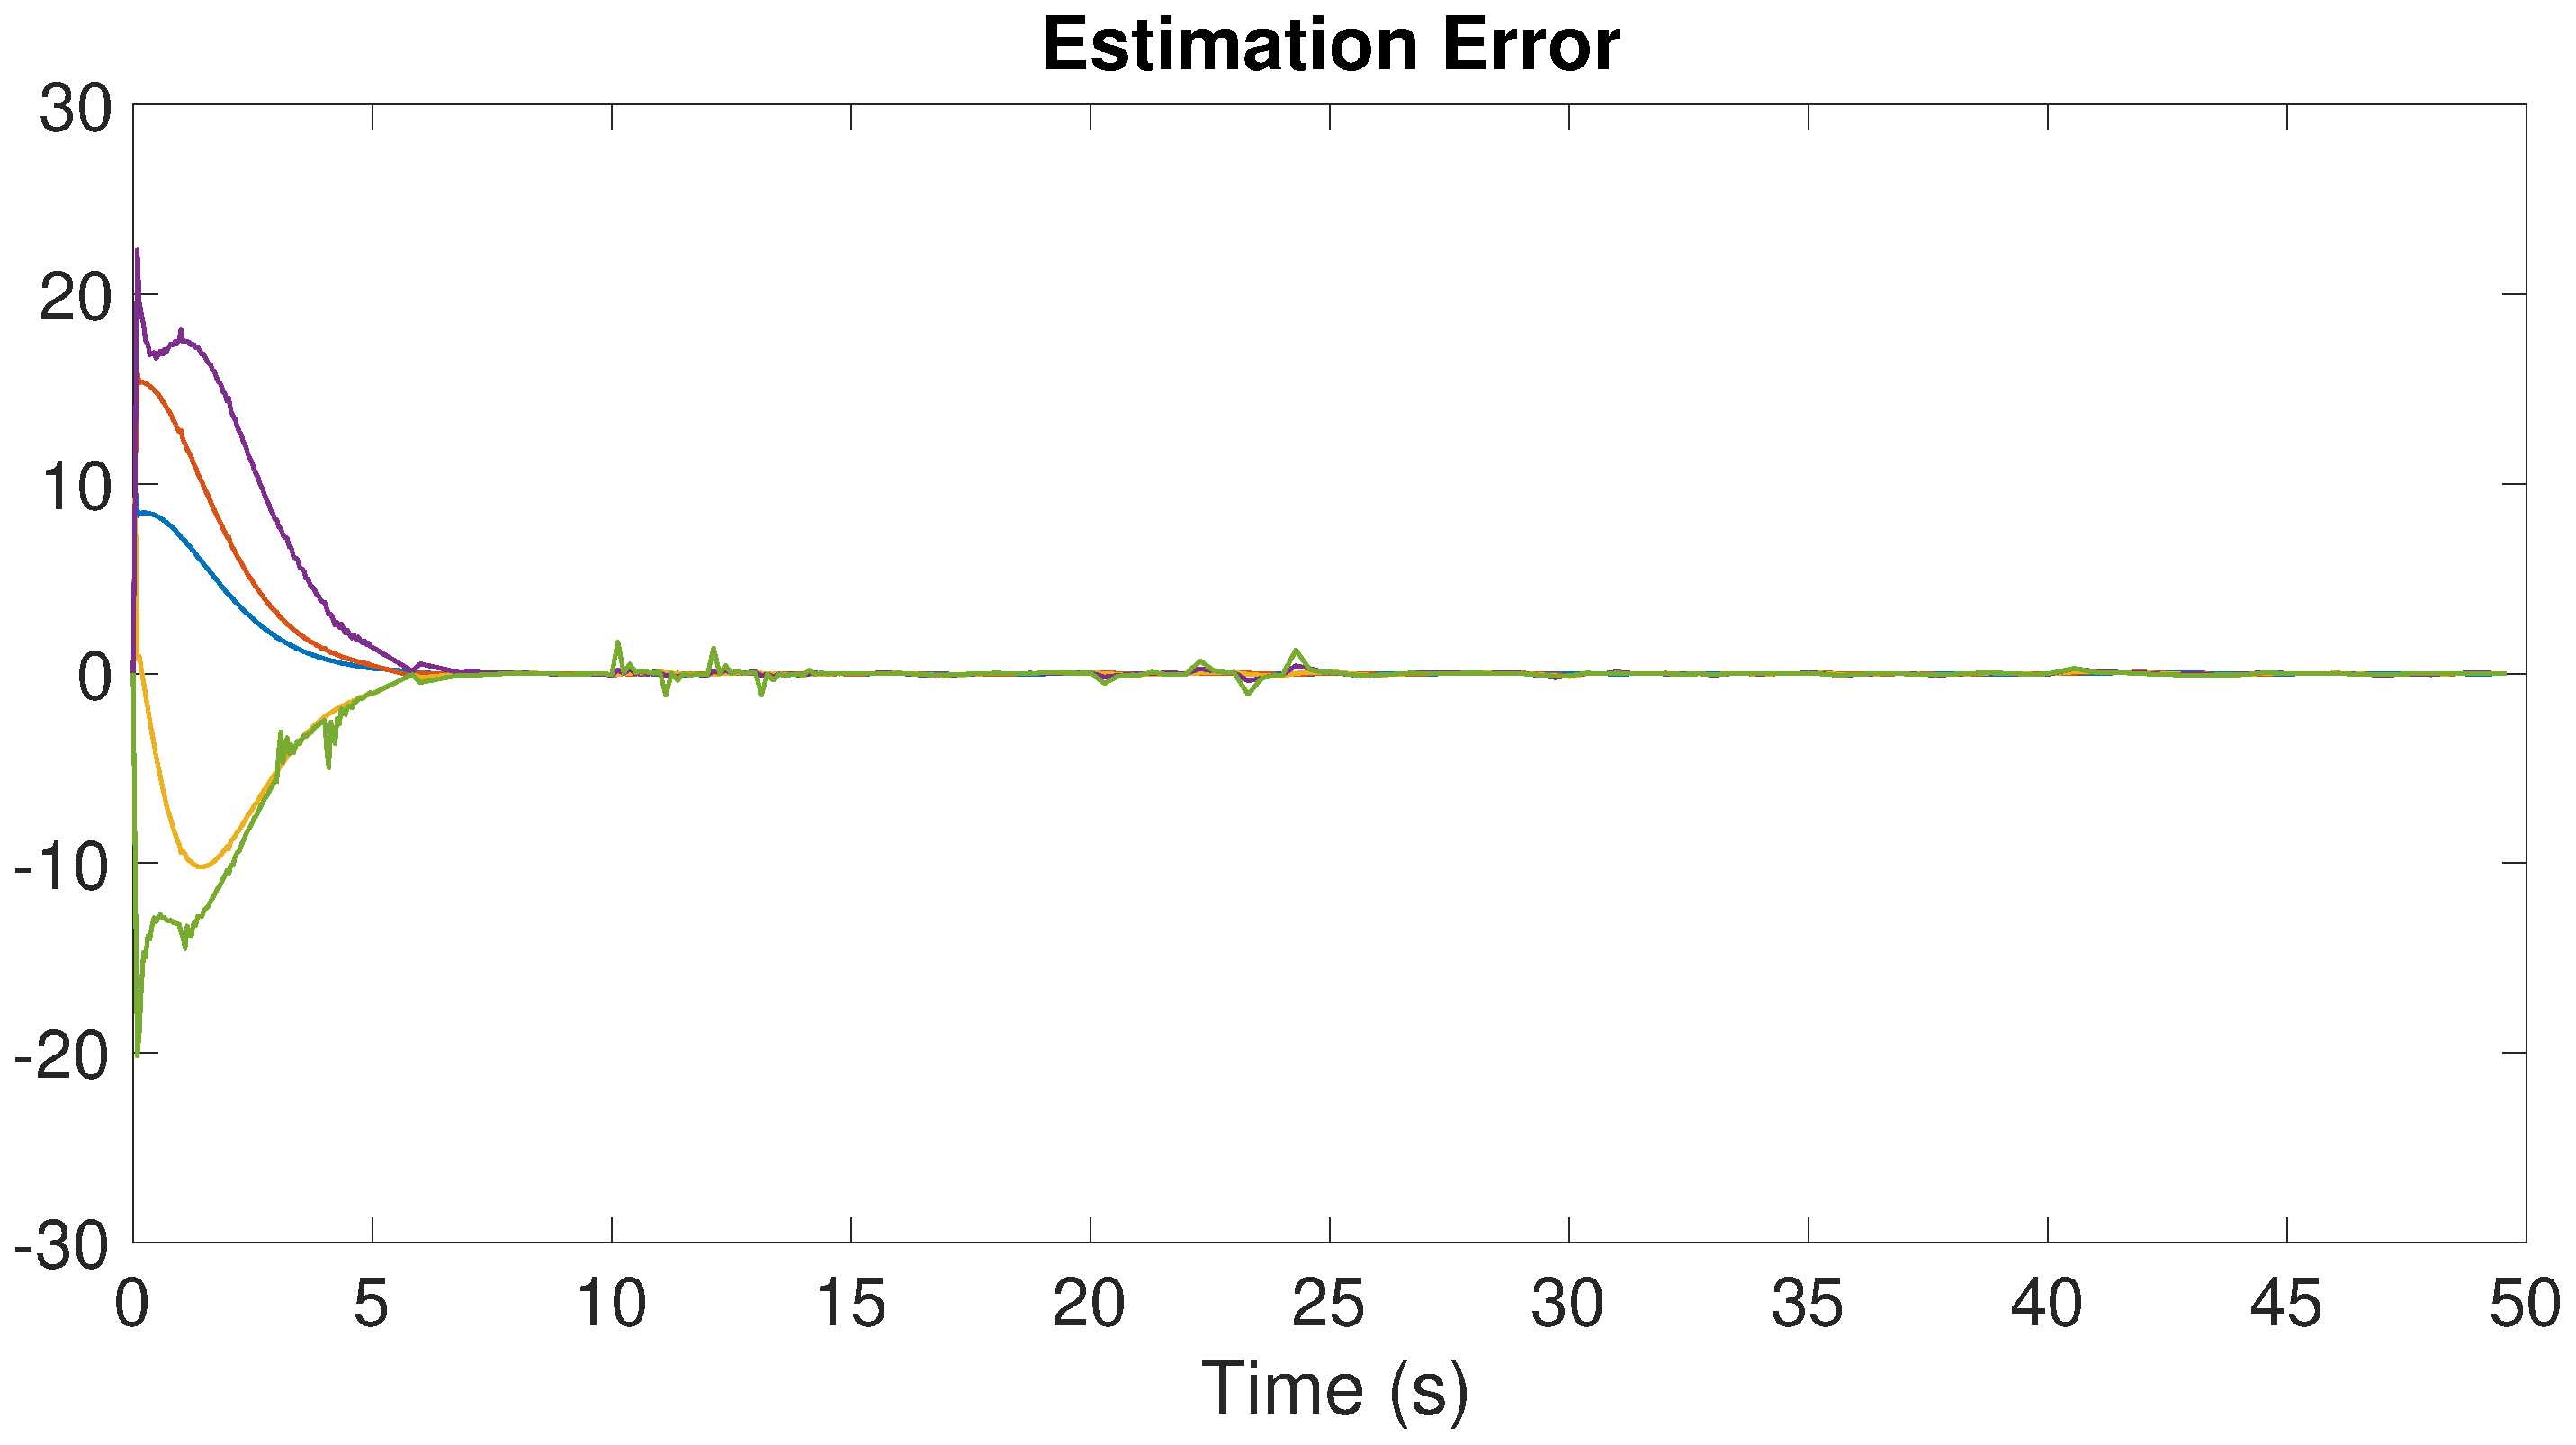
\includegraphics[width=\linewidth]{stair-input-error}
        \caption{Estimation error.}%
      \end{figure}
    \end{column}%
  \end{columns}
\end{slide}

\begin{slide}{Results}
  \begin{columns}[c]
    \begin{column}{0.55\textwidth}
      \begin{figure}[ht!]
        \centering
        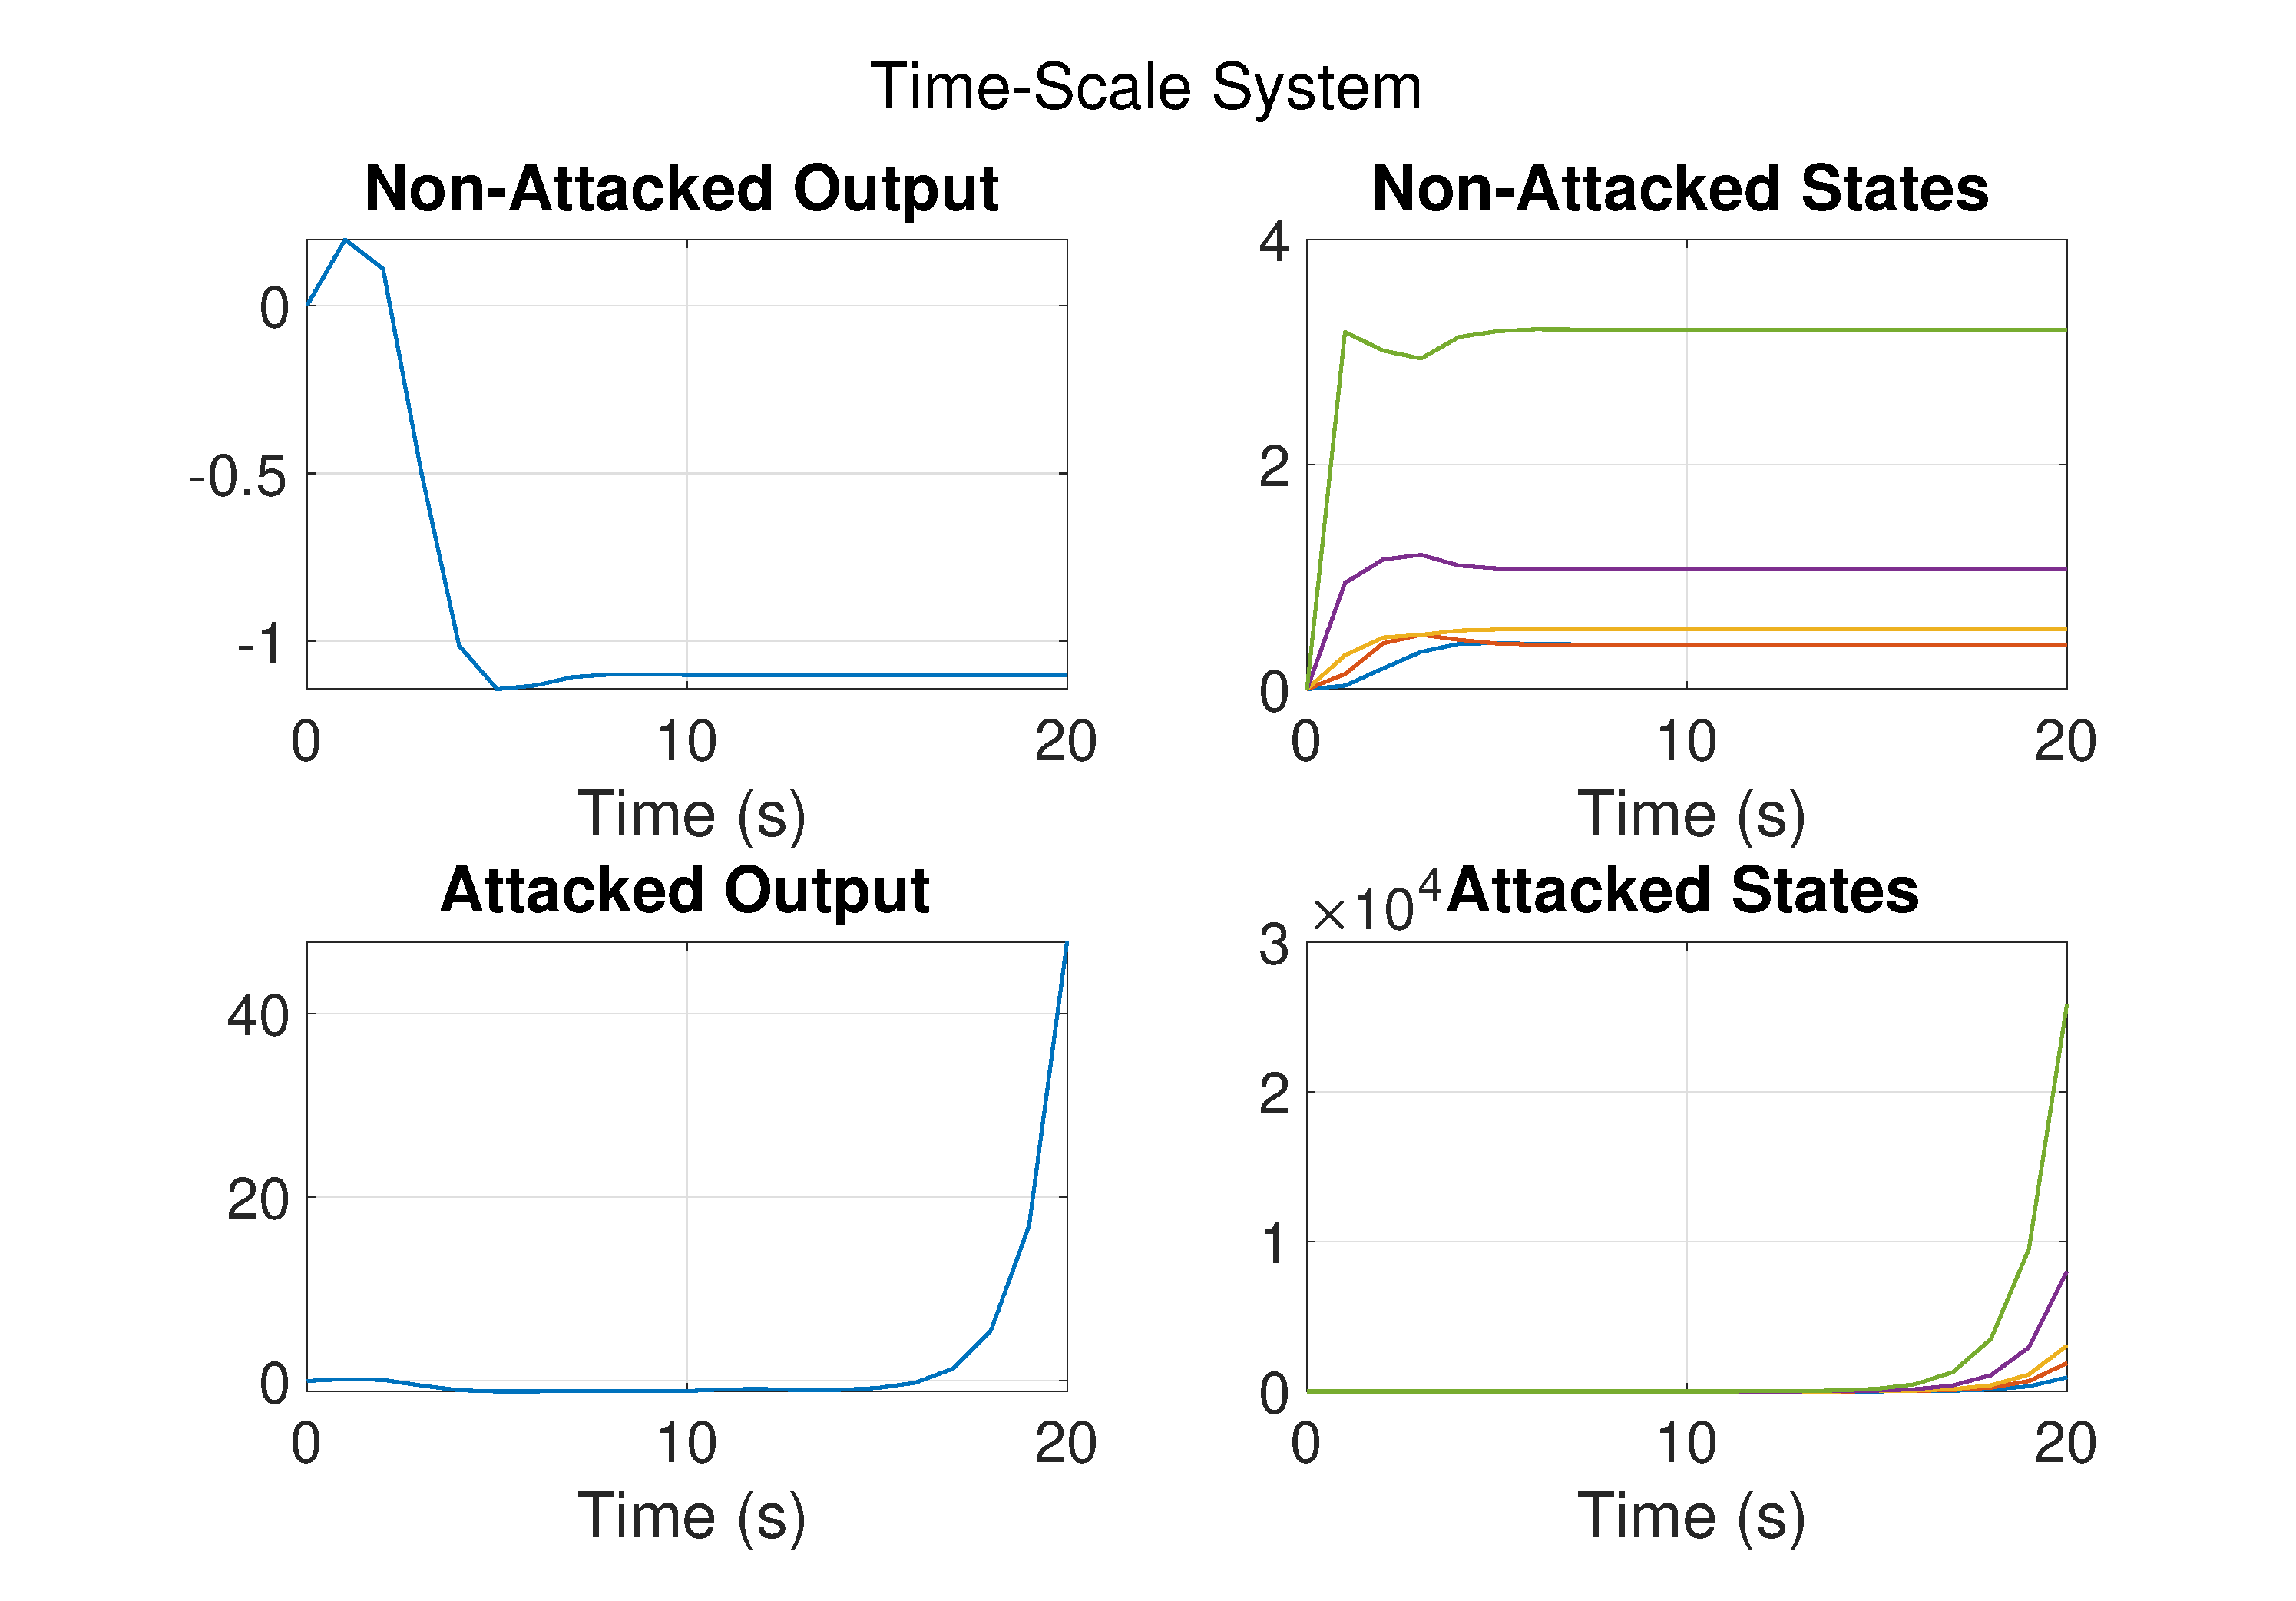
\includegraphics[width=\linewidth]{ts-system}
        \caption{Time-scale system's observer with \(\mu=\SI{1}{\second}\).}%
      \end{figure}
    \end{column}%
    \hfill%
    \begin{column}{0.55\textwidth}
      \begin{figure}[ht!]
        \centering
        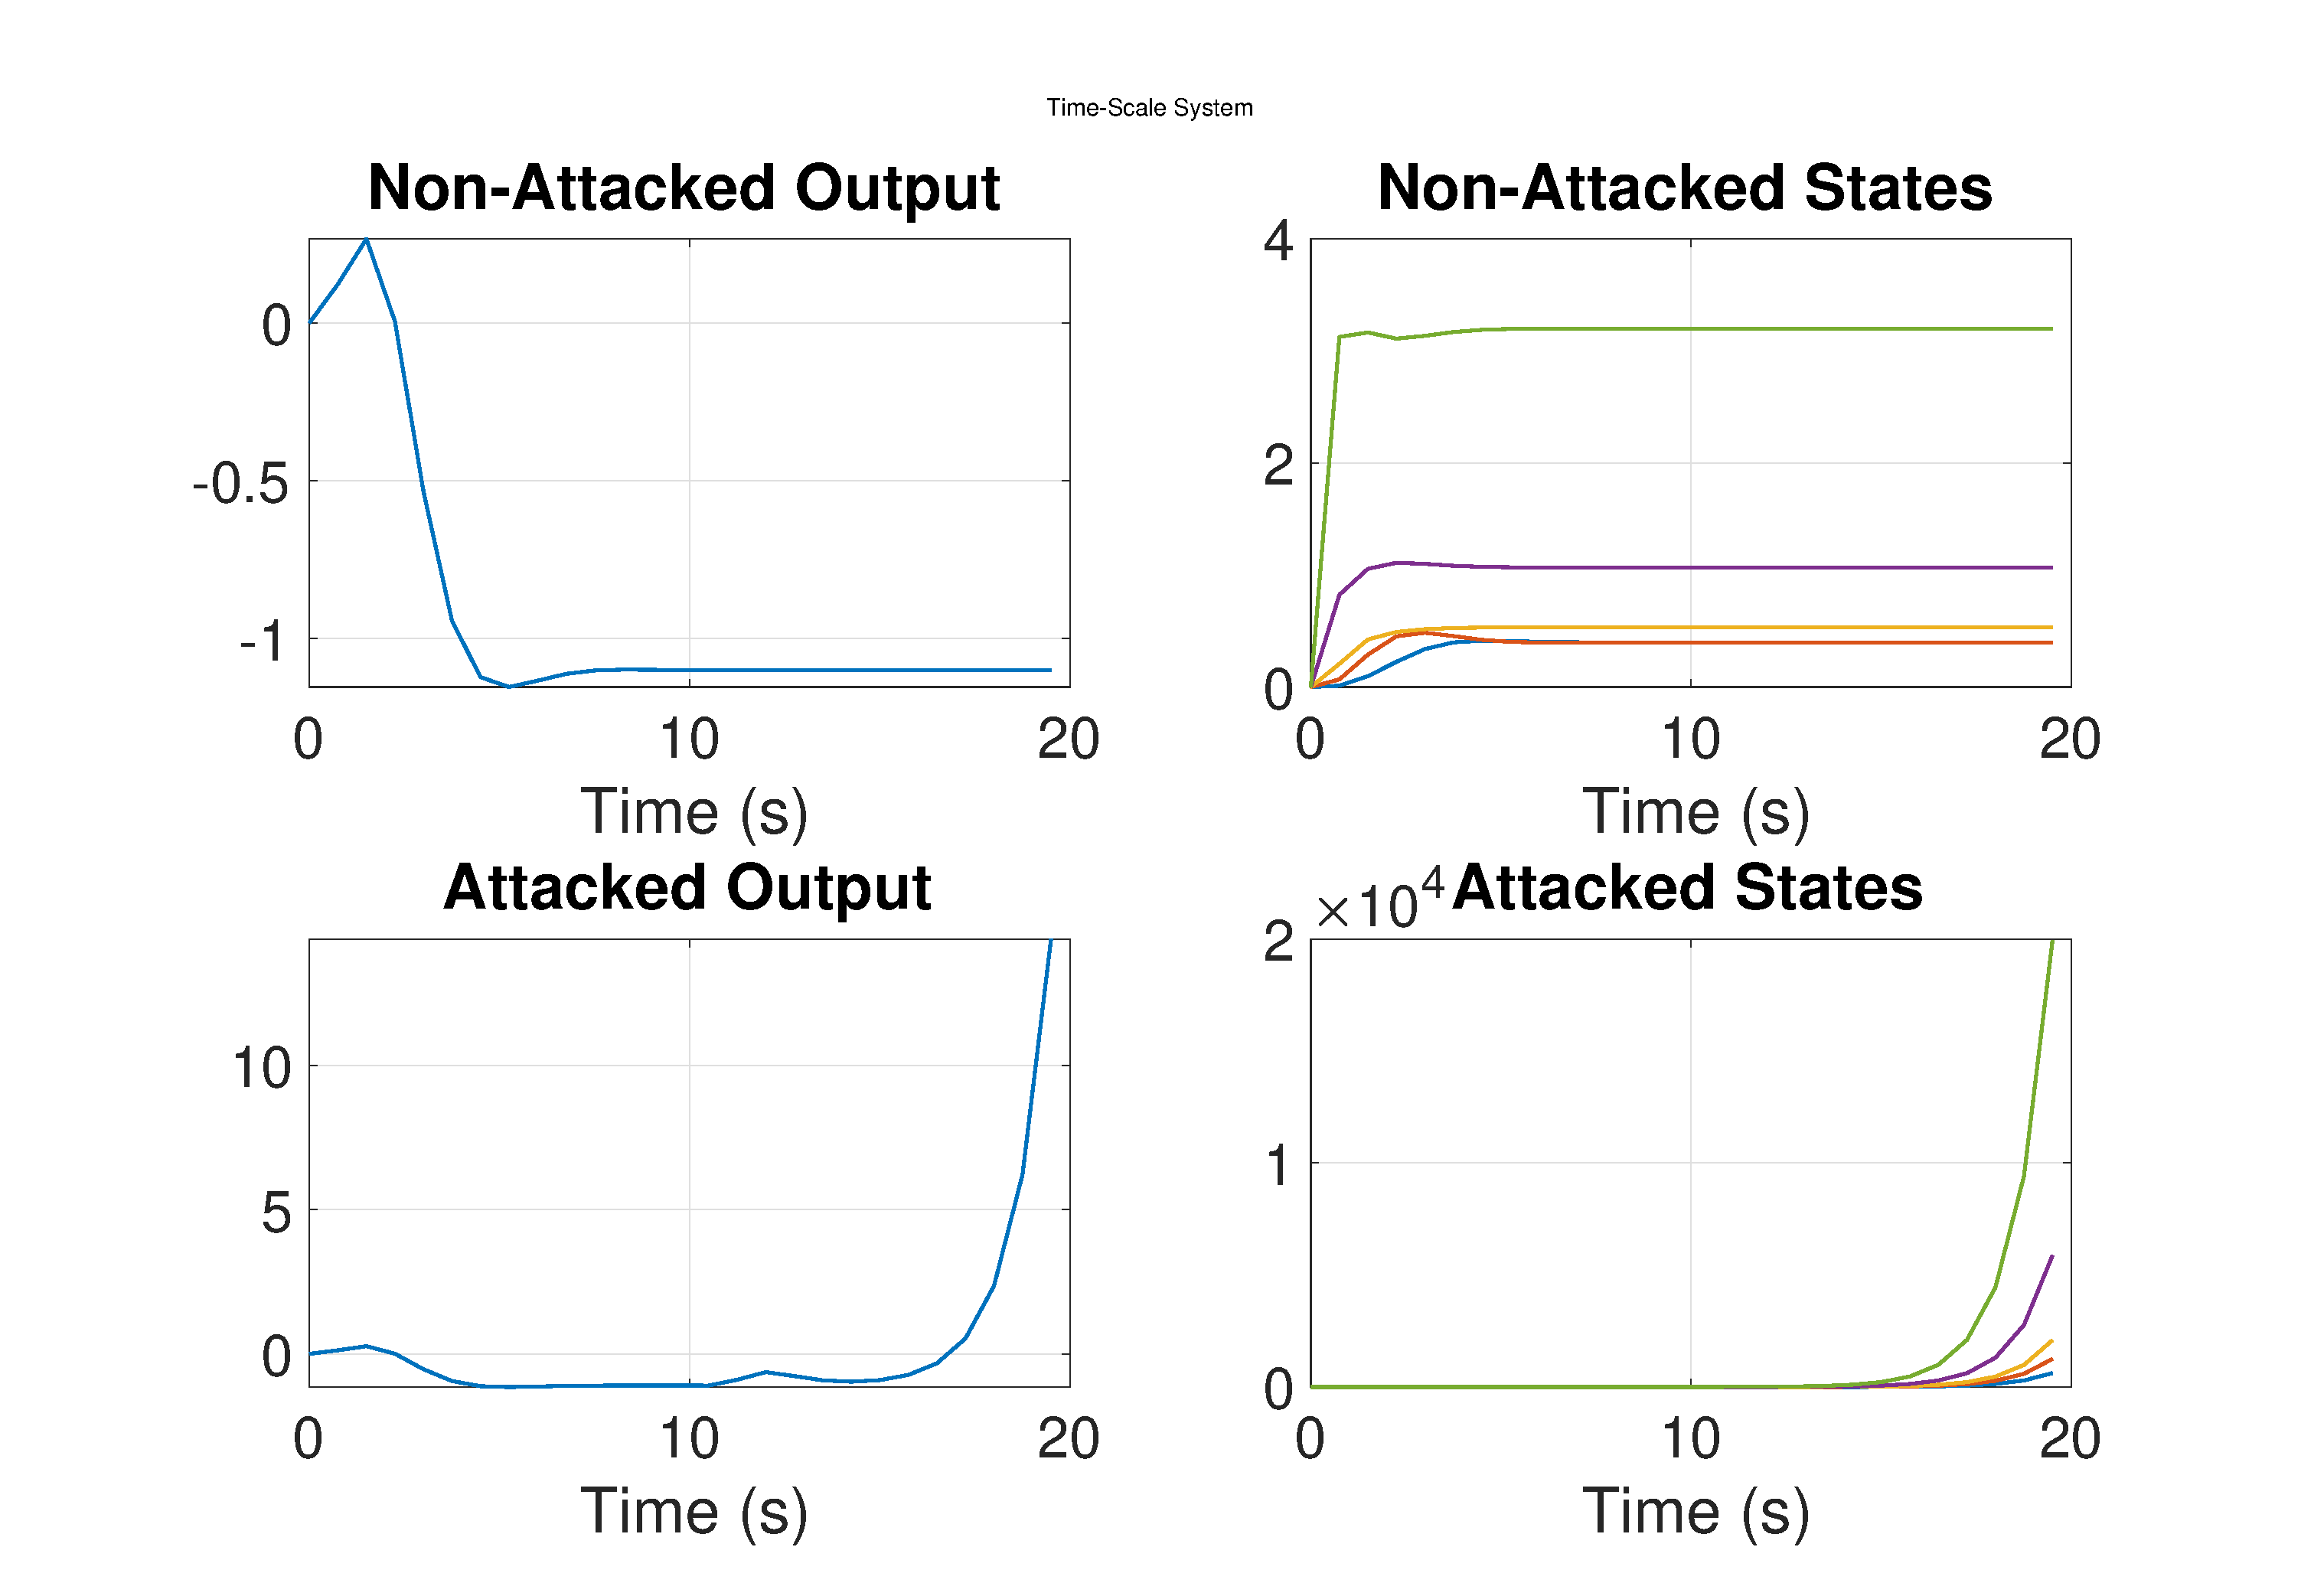
\includegraphics[width=\linewidth]{ts-system2}
        \caption{Time-scale system's observer with \(\mu=\SI{0.75}{\second}\).}%
      \end{figure}
    \end{column}%
  \end{columns}
\end{slide}
